\documentclass[12pt]{article}
\usepackage{ctex}
\usepackage[english]{babel}
\usepackage{blindtext}
\usepackage{nameref}
\usepackage{fancyhdr}
\usepackage{amsmath,amssymb,amsthm}
\usepackage{graphicx,float}
\usepackage{physics}
\usepackage{pgfplots}
\usepackage[a4paper, total={6in, 9in}]{geometry}

\graphicspath{{../images/}}

\pagestyle{fancy}
\fancyhf{}
\fancyhf[FL]{Mok-DSE-MATH-CP}
\fancyhf[CF]{\thepage}

\newcommand{\innerprod}[2]{\langle{#1},{#2}\rangle}
\newcommand{\id}{\mathtt{id}}

\newtheorem*{definition}{Definition}
\newtheorem*{theorem}{Theorem}
\newtheorem*{corollary}{Corollary}
\newtheorem*{lemma}{Lemma}
\newtheorem*{proposition}{Proposition}
\newtheorem*{remark}{Remark}
\newtheorem*{claim}{Claim}
\newtheorem*{example}{Example}
\newtheorem*{axiom}{Axiom}

\begin{document}
    \thispagestyle{plain}

    \centering 

    \section*{HKDSE MOCK EXAM PAPER\\MATHEMATICS Compulsory Part\\Question-Answer Book\\Set 1}

    Time allowed: 2 hours 15 minutes

    Name:\hrulefill \hfill Marks:\hrulefill/105

    \raggedright

    \subsection*{Instructions}

    \begin{enumerate}
        \item This paper must be answered in English.
        \item Unless otherwise specified, all working must be clearly shown.
        \item Unless otherwise specified, numerical answers must be exact.
        \item This paper is for \textbf{internal use} only.
        \item All questions are constructed by Mok Owen.
        \item The mock paper is composed of 3 parts, including Section A(1), Section A(2) and Section B. Each part consist of 35 marks each.
    \end{enumerate}

    \newpage


    \begin{enumerate}
        \subsection*{Section A(1) (35 marks)}
        \item Simplify $\dfrac{(m^3n^{-2})^3}{(m^{-1}n^7)^{-2}}$ and express your answer with positive indices.\hfill (3 marks)
        \item Make $a$ the subject of the formula $\dfrac{a+1}{a-1}=\dfrac{b+c}{d-c}$.\hfill (3 marks)
        \item Factorize \begin{enumerate}
            \item $4x^2+4xy+y^2$,
            \item $12x^2+xz+z^2$,
            \item $(4x^2+4xy+y^2)-(12x^2+xz+z^2)$.
        \end{enumerate}\hfill (3 marks)
        \item Given that $a:b=5:6$ and $2b=3c$.\begin{enumerate}
            \item Find $a:b:c$.
            \item Find the value of $\dfrac{9a+2b+3c}{a+b+c}$.
        \end{enumerate}\hfill (3 marks)
        \item Given a stock X in the market at \$x per unit at instance. It is known that a person could buy a certain amount of stock X at this price level. What is the percentage change in amount affordable for that person if the stock price is increased by 20\% ?\hfill (4 marks)
        \item Consider the compound inequality \begin{align*}
            \begin{cases}
                \dfrac{x}{x+1}\leq 5\\
                3x+2\leq 0
            \end{cases}
        \end{align*}
        \begin{enumerate}
            \item Solve the inequality system.
            \item Write down the number of integers satisfying the inequality.
        \end{enumerate}\hfill (4 marks)
        \item Let $f(x)=x^2-kx-(k+1)$ has equal roots. Find \begin{enumerate}
            \item $k$,
            \item the possible y-intercepts of $y=kf(x)$.
        \end{enumerate}\hfill (5 marks)
        \item Given the following figure \begin{figure}[H]
            \centering
            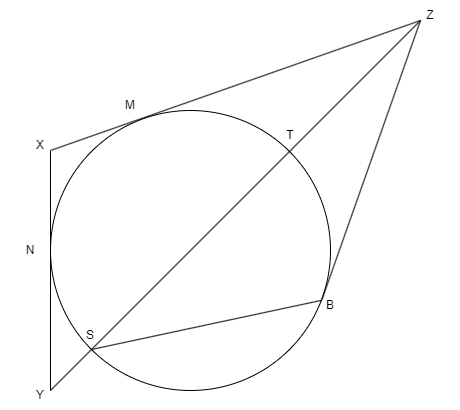
\includegraphics[scale=0.6]{geometry1.png}
        \end{figure}
        Suppose ST is the diameter of the circle passing through S,N,M,T,B. Assume XMZ and XNY are tangent to the circle. Further assume ZB is a tangent to the circle, while $\angle TSB = 30^\circ$ and $\angle NYS = 45^\circ$. Let the center of the circle be O. Find the value of $\angle MON$. \hfill (5 marks)
        \item The following stem-and-leaf diagram shows the distribution of the ages of Tommy's girlfriends:\begin{table}[htbp]
            \centering
            \begin{tabular}{r|l@{\hspace{4 pt}}l@{\hspace{4 pt}}l@{\hspace{4 pt}}l@{\hspace{4 pt}}l@{\hspace{4 pt}}l@{\hspace{4 pt}}l@{\hspace{4 pt}}l@{\hspace{4 pt}}l@{\hspace{4 pt}}l@{\hspace{4 pt}}l@{\hspace{4 pt}}}
                Stem & \multicolumn{10}{l}{ Leaf}\\
                \hline
                0&6&6&7&8&9&9\\
                1&0&0&1&5&5&5&5&7&8&9\\
                2&2&3&7\\
                3&0&b
            \end{tabular}
            \end{table}

        It is known that the range of the distribution is over 30.
        \begin{enumerate}
            \item Is it possible to have mean of the distribution to be less than 15.6? Explain your answer briefly.
            \item Suppose the current mean is maximized. Compute the standard deviation of the distribution.
        \end{enumerate} \hfill (5 marks)

        \subsection*{Section A(2) (35 marks)}
        
        \item It is given that $f(x)$ is composed of 3 parts. The first part varies as constant. The second part and the third part varies directly and inversely with $x$ respectively. Suppose that $f(1)=f(-1)$, $2f(2)=5$ and $4f(4)=19$.\begin{enumerate}
            \item Solve $f(x)=1$. \hfill (3 marks)
            \item Define $g(x)=xf(x)-1$ and denote the graph of $y=g(x)$ by $G$. Denote $G$'s x-intercepts by $X$ and $Y$, where $X$ is on the left of $Y$, and the vertex of $G$ by $V$. Find the area of $\triangle VXY$. \hfill (3 marks)
        \end{enumerate}

        \item The table below shows the distribution of the range of years of sentence of prisoners in a certain jail.
        \begin{center}
            \begin{tabular}{||c||c|c|c|c||}
                \hline
                Years of sentence & 1 - 10 & 11 - 20 & 21 - 30 & 31 - 40\\
                \hline
                Number of prisoners & 109 & 75 & $n$ & $n$ - 10\\
                \hline
            \end{tabular}
        \end{center}
        It is given that the expected years of sentence in the jail is 17.5 years if a random prisoner is chosen.\begin{enumerate}
            \item Find the median group and mode group of the distribution. \hfill (4 marks)
            \item Tommy was one of the prisoners in this jail with less than 10 years of sentence. During period of sentence, he murdered 3 prisoners whose years of sentence are below 10 years. He then received an extension of sentence. The mean of the new distribution is nearly unchanged. In what range of years of sentence should Tommy be extended to? \hfill (3 marks)
        \end{enumerate}

        \item Given that $f(x)$ is a polynomial such that $(x-1)f(x)$ is divisible by $x^2+x+1$.\begin{enumerate}
            \item Show that $f(x)$ is divisible by $x^2+x+1$. \hfill (3 marks)
            \item Consider $g(x)$ is a polynomial such that $f(x)$ is a factor of $g(x)$. Someone claims that if $(x-1)g(x)$ is divisible by $x^3$ then $g(x)$ is at least of degree 5. Is the claim correct? Explain your answer. \hfill (4 marks)
        \end{enumerate}
    \end{enumerate}

\end{document}